\documentclass[10pt,a4paper]{beamer}
\usepackage[spanish]{babel}
\usepackage[utf8]{inputenc}
\usepackage{amsmath}
\usepackage{amsfonts}
\usepackage{listings}
\usepackage{amssymb} 
\usetheme{Madrid} 
\usepackage{hyperref}

\author{Marasca, Rodríguez, Di Pietro, Scally} 
\title{HTTPSpy} 
\institute{FCEN, UBA} 
 
\begin{document} 

\maketitle

\begin{frame}
	\frametitle{Objetivos iniciales}
	\begin{block}{Objetivo inicial}
	Se deberá implementar un sniffer http que permita escuchar el tráfico hacia un proxy http, para luego facilitar el análisis del tráfico capturado.
	\end{block}
	Características:
	\begin{itemize}
		\item El tráfico deberá almacenarse en una base de datos SQL.
		\item Proveerá una interfaz para realizar consultas sobre la base de datos.
		\item Se almacenará ip-origen, fecha y hora, método http, URL.
		\item De ser posible se almacenarán los headers de la respuesta, incluyendo código de respuesta, tamaño de la misma y Content-Type.
		\item Se podrán generar reportes de anomalías.
	\end{itemize}
\end{frame}

\begin{frame}

	\frametitle{Objetivos adicionales}
	Objetivos adicionales:
	\begin{itemize}
		\item Se podrá filtrar el tráfico a almacenar según reglas ingresadas por el usuario (hosts, puertos, etc.).
		\item El usuario podrá seleccionar que parte de la conversación HTTP desea almacenar (hosts, puertos, método, headers, etc.).
		\item Podrán utilizarse diferentes formas de almacenar el tráfico sniffeado (SQL, texto plano, XML, YAML, etc.).
		\item La herramienta deberá ser robusta y no romperse por anomalías en el tráfico.
		\item Será deseable que se trate de utilizar sólo herramientas/módulos estándares del lenguaje seleccionado para su implementación.
		\item Deberá ser un sistema muy simple y poco acoplado, de forma de permitir que se utilice para implementar sistemas más complejos.
		\item La implementación será compacta y portable.
	\end{itemize}
	
\end{frame}

\begin{frame}[fragile]
	\frametitle{Request HTTP}
	{\small
	\begin{verbatim}
GET / HTTP/1.1
User-Agent: Mozilla/4.0 (compatible; MSIE 6.0; Windows NT 5.0) Opera 7.11  [en]
Host: 10.1.1.1
Accept: text/xml,application/xml,application/xhtml+xml,text/html
Accept-Language: en
Accept-Charset: windows-1252, utf-8, utf-16, iso-8859-1;q=0.6, *;q=0.1
Accept-Encoding: deflate, gzip, x-gzip, identity, *;q=0
Connection: Keep-Alive
	\end{verbatim}
	}
\end{frame}

\begin{frame}[fragile]
	\frametitle{Response HTTP}
	{\small
	\begin{verbatim}
HTTP/1.1 200 OK
Date: Sat, 20 Nov 2004 10:21:06 GMT
Server: Apache/2.0.40 (Red Hat Linux)
Last-Modified: Mon, 08 Mar 2004 20:27:54 GMT
ETag: "46eed-a0-800ce680"
Accept-Ranges: bytes
Content-Length: 160
Connection: close
Content-Type: text/html; charset=ISO-8859-1

<html>
	<head>
	<title>Y la triple corona?</title>
	</head>
	<body>
	...
	</body>
</html>
	\end{verbatim}
	}
\end{frame}

\begin{frame}[fragile]
	\frametitle{Request HTTPS}
	{\small
	\begin{verbatim}
CONNECT www.google.com:443 HTTP/1.0
User-Agent: Mozilla/5.0 (X11; Ubuntu; Linux i686; rv:13.0) Firefox/13.0.1
Host: www.google.com
Content-Length: 0
Proxy-Connection: Keep-Alive
	\end{verbatim}
	}
\end{frame}

\begin{frame}[fragile]
	\frametitle{Response HTTPS}
	{\small
	\begin{verbatim}
.........|ia..R..Z*..j.$....Z.X$g/D46.\.]...j
J.[.C...x*=..%...%^.8m.....%c.. ..5...~./.]..z...e.}...|
.v.......+.[.v....#qC.x.d....GK...B`.KM1)]...21...;..
T%.......(.......).d.......U........V...W.u..dB...Lz..!.?...x
...9....S.......nI.y..;.v.,..P...
S..xl^^T...._~"Y..5..V...X".%........a....C?.....-..<...
.n..e... h.1.f.0-?.....a..|Ygy8H.u.l-d...S...<.......z.c.
.....J...1>..L.....6u..b&...QV|1.5.q....x?Y..E.6..
........1.+.....^.h......4."..H..i...Pk...
.F6.._xR.X.j....E.A...2<'b...N$.[.<Q;^w......_K.]..,.
./.j.@........'...rC...w}.. ....9.D..ii+.:w;.....
......'..w.c3g.......f.....
..i..N.L......vjE.....M.~..B.Al
..........q.V.yQ3/J...
	\end{verbatim}
	}
\end{frame}


\begin{frame}
	\frametitle{Herramientas analizadas}
	Se analizaron las siguientes tecnologias para la implementación del proyecto.
	\begin{itemize}
		\item Lenguajes: Python, C/C++, Java, Perl.
		\item libpcap, pycap, scapy.
		\item libnids, pynids.
		\item http\_parser.
		\item MySql, SQLite, PostgreSql, Oracle, Sql Server, SQLAlchemy.
		\item Mojolicious, Djando, Bottle, Web2py.
		\item ncurses.
		\item tinyproxy.
	\end{itemize}
	
\end{frame}


\begin{frame}

	\frametitle{Herramientas utilizadas}
	Para el desarrollo utilizamos las siguientes tecnologías.
	\begin{itemize}
		\item Lenguajes: Python
		\item Sniffing: pynids.
		\item Parser: http\_parser.
		\item Almacenamiento: SQLite.
		\item Framework Web: Mojolicious.
		\item Auxiliares: tinyproxy, tcpdump, wireshark, etc.
	\end{itemize}
	
\end{frame}


\begin{frame}

	\frametitle{Deploy}
	\begin{figure}[hbtp]
		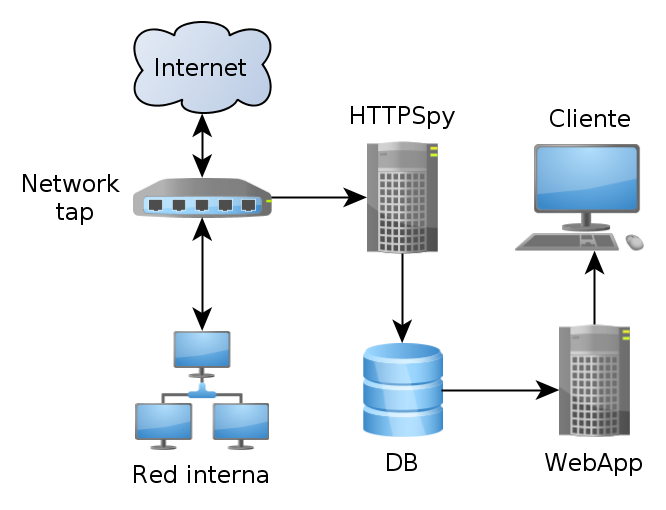
\includegraphics[scale=0.3]{img/deploy.png}
	\end{figure}
	\begin{center}
		\large{Ejemplo de deploy}
	\end{center}
	
\end{frame}	

\begin{frame}

	\frametitle{Diseño de la aplicación}

	\begin{figure}[hbtp]
		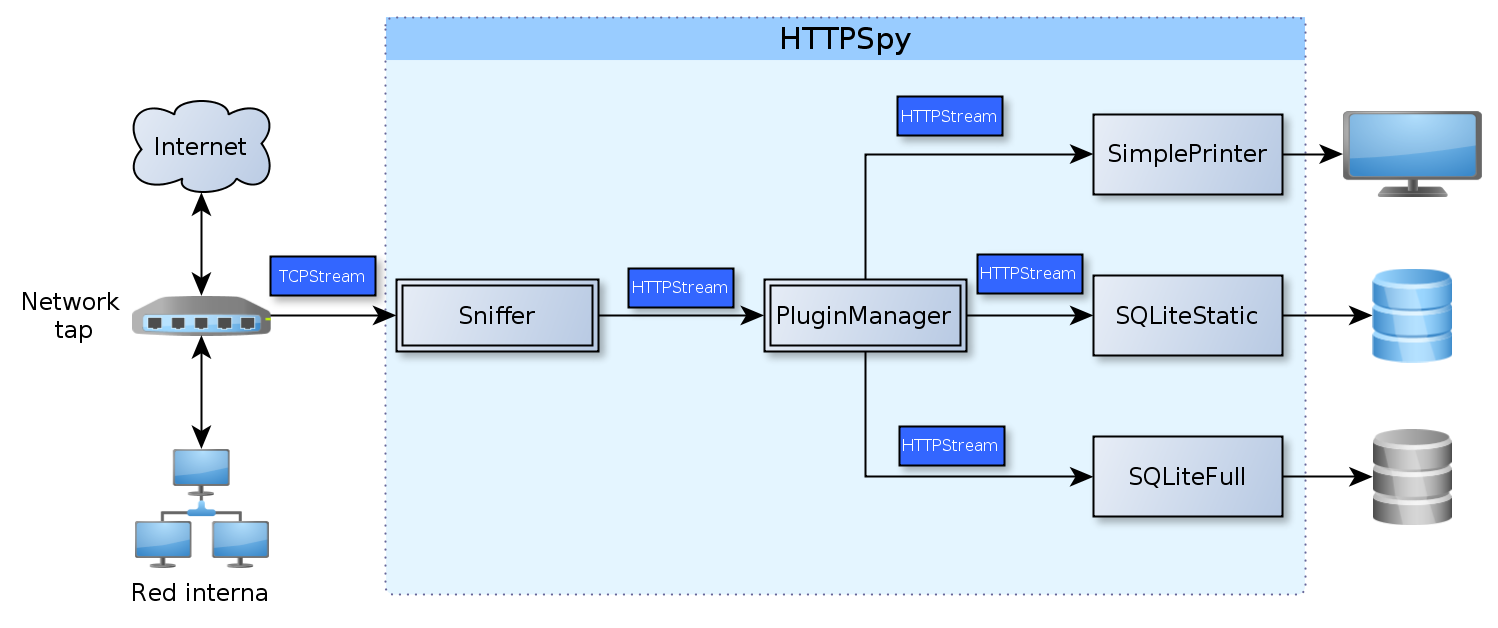
\includegraphics[scale=0.22]{img/modelo.png}
	\end{figure}

\end{frame}

\begin{frame}

	\frametitle{HTTPSniffer}
	\begin{block}{Responsabilidad}
		Encargado de capturar el tráfico según las reglas de filtrado definidas.
		Por cada conversación HTTP genera una instacia de HTTPStream y ejecuta la función de callback pasándolo como parámetro. Es un singleton que encapsula a la librería pynids.
	\end{block}
	\begin{figure}[hbtp]
		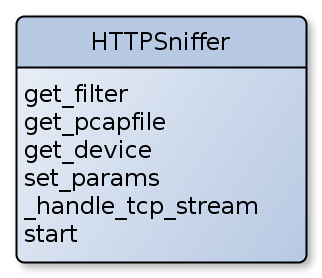
\includegraphics[scale=0.40]{img/HTTPSniffer.png} 
	\end{figure}
\end{frame}

\begin{frame}

	\frametitle{HTTPStream}
	\begin{block}{Responsabilidad}
		Representa una conversacion HTTP, almacena toda la información interesante sobre la misma. No alacena el payload de la conversación.
	\end{block}
	\begin{figure}[hbtp]
		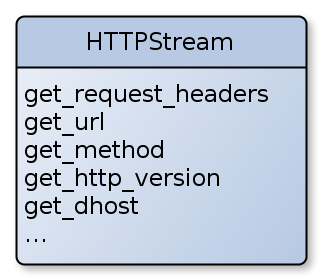
\includegraphics[scale=0.40]{img/HTTPStream.png} 
	\end{figure}
\end{frame}


\begin{frame}

	\frametitle{PluginsManager}
	\begin{block}{Responsabilidad}
		Administra los plugins instalados en la aplicación. Asocia el nombre del plugin con la clase correspondiente. 
	\end{block}
	\begin{figure}[hbtp]
		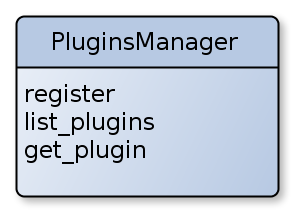
\includegraphics[scale=0.40]{img/PluginsManager.png} 
	\end{figure}
\end{frame}

\begin{frame}

	\frametitle{Plugins}
	\begin{block}{Responsabilidad}
		Son los encargados de procesar los requests capturados por el sniffer. Cada uno debe implementar los métodos log\_stream y help. 
	\end{block}
	\begin{figure}[hbtp]
		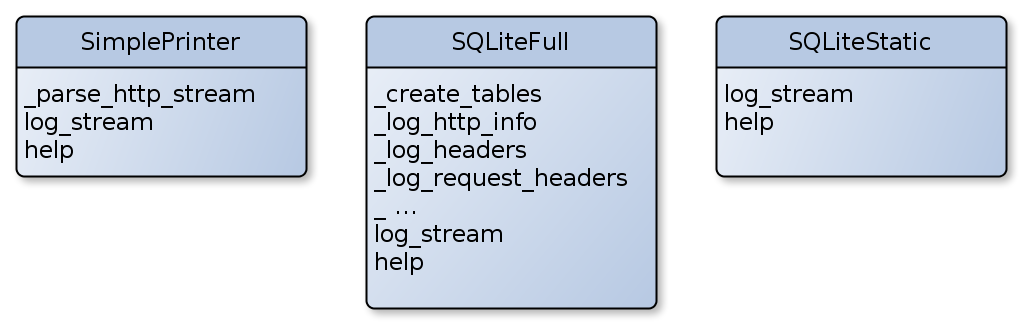
\includegraphics[scale=0.30]{img/Plugins.png} 
	\end{figure}
		
\end{frame}

\begin{frame}

	\frametitle{Plugins implementados}
	\begin{block}{SimplePrinter}
		Este plugin imprime por stardard output, según un formato configurable, información sobre la conversacion HTTP.
	\end{block}
	\begin{block}{SQLiteStatic}
		Almacena en una unica tabla SQLite los siguientes campos: source host, destination host, request path, request method, status code, content length, content type.
	\end{block}
	\begin{block}{SQLiteFull}
		Almacena en tres tablas SQLite toda la información relacionada a la conversación, incluyendo todos los headers.
	\end{block}

\end{frame}

\begin{frame}
	\frametitle{Instalación Debian likes}
	\begin{block}{Repositorio tentativo}
		\url{https://github.com/cdipietro/2012\_1c\_seginfo}	
	\end{block}
	Instalación paso a paso:
	\begin{enumerate}
		\item apt-get install python python-pip python-dev python-nids
		\item pip install http\_parser
		\item cpan App::cpanminus
		\item cpanm DBI DBD::SQLite Mojolicious
		\item Enjoy!	
	\end{enumerate}
	
\end{frame}

\begin{frame}[fragile]
	\frametitle{Modo de uso}
	{\small
	\begin{verbatim}
	usage: main.py [-h] [--pcapfile PCAPFILE | --device DEVICE] 
	[--filter FILTER]
	[--list-plugins | --help-plugin HELP_PLUGIN | --plugins PLUGINS]

A very basic http sniffer

optional arguments:
  -h, --help            show this help message and exit
  --pcapfile PCAPFILE   read a tcp stream from a file
  --device DEVICE       set the device to sniff
  --filter FILTER       set the filter (see man tcpdump)
  --list-plugins        List availables plugins
  --help-plugin HELP_PLUGIN
                        Show help for a plugin
  --plugins PLUGINS     File with configured plugins


	\end{verbatim}
	}
\end{frame}

\begin{frame}[fragile]
	\frametitle{Ejemplo de uso}
	printer.yml:
	{\small
	\begin{verbatim}
- name      : SimplePrinter
  delimiter : "\t"
  format    : "shost method >Host path status_code <Content-Type"
    \end{verbatim}
    }
    Comando para capturar de un dispositivo:
    {\small
	\begin{verbatim}
	$python main.py --device eth0 --plugins printer.yml
	\end{verbatim}
	}
    Comando para procesar un pcapfile:
    {\small
	\begin{verbatim}
	$python main.py --pcapfile trafico.pcap --plugins printer.yml
	\end{verbatim}
	}
	Salida:
    {\small
	\begin{verbatim}
	192.168.0.12	GET	www.gnu.org	/	200	text/html
	\end{verbatim}
	}
	    
\end{frame}



\begin{frame}

	\frametitle{Demo de plugins}
	\begin{figure}[hbtp]
		
\includegraphics[scale=0.4]{img/demo.jpg}
	\end{figure}
	\begin{center}
		\huge{Demo}
	\end{center}
	
\end{frame}

\begin{frame}[fragile]

	\frametitle{Interfaz Web}
	\begin{block}{}
		Es una pequeña aplicación web que permite realizar consultas predefinidas sobre la base de datos generada por el sniffer. 
	\end{block}
	
	\begin{enumerate}
		\item Los informes preconfigurados se definen mediante un archivo de configuración con formato yaml.
		\item Se pueden definir informes parametrizados.
		\item Aún se encuentra en fase de desarrollo.
	\end{enumerate}
	Ejemplo: 
	{\small
	\begin{verbatim}
	- nombre: Listar fecha, origen, destino (like)
  query: 'SELECT date, shost, host FROM http_log WHERE host LIKE ?'
  campos: 
   - Destino
  columnas:
   - Fecha
   - Origen
   - Destino

	\end{verbatim}
	}
	
\end{frame}

\begin{frame}

	\frametitle{Demo de la Interfaz Web}
	\begin{figure}[hbtp]
		
\includegraphics[scale=0.4]{img/demo.jpg}
	\end{figure}
	\begin{center}
		\huge{Demo}
	\end{center}
	
\end{frame}

\begin{frame}
	\frametitle{Mejoras a Futuro}
	\begin{itemize}
	
	\item Mejorar la robustez de la Interfaz web.
	\item Programar una interfaz basada en ncurses.
	\item Programar más tests de unidad.
	\item Pruebas de performance en ambientes productivos de gran escala.
	\item Plugin de Syslog.
	\item Plugin Oracle, PostgreSQL, Mysql y SQLServer o SQLAlchemy.
	\item Script de instalación.
	\item Mejorar la documentación.
	\item Reestruturar el código para subirlo a "Python Package Index".
	\item Crear un repositorio y una web para la aplicación (wiki + bugtracker).

	\end{itemize}
	

\end{frame}


\begin{frame}

	\frametitle{Preguntas}
	\begin{figure}[hbtp]
		
\includegraphics[scale=0.5]{img/preguntas.png}
	\end{figure}
	\begin{center}
		\huge{¿Preguntas?}
	\end{center}
	
\end{frame}

\begin{frame}

	\frametitle{Fin}
	\begin{figure}[hbtp]
		
\includegraphics[scale=0.15]{img/gracias.jpg}
	\end{figure}
	\begin{center}
		\huge{Gracias}
	\end{center}
	
\end{frame}

\end{document}
